\documentclass{article}

% chinese fonts
\usepackage{ctex}

% math fonts
\usepackage{amsmath}
\usepackage{amsthm}
\usepackage{amssymb}
\usepackage{bm}

% figures
\usepackage{tikz}
\usepackage{graphicx}
\graphicspath{{./figures/}}

% tables
\usepackage{tabularx}
\usepackage{booktabs}
\usepackage{multirow}

% codes
\usepackage{listings}
\lstset{language     = Matlab,
        basicstyle   = \ttfamily,
        keywordstyle = \color{cyan},
        rulecolor    = \color{black},
        commentstyle = \color{green},
        keepspaces   = true,
        tabsize      = 4,
}

% hyperlinks
\usepackage{hyperref}
\hypersetup{
  breaklinks,
  colorlinks = true,
  citecolor  = blue,
  linkcolor  = red,
  urlcolor   = magenta,
}

% algorithms
\usepackage{algorithm}
\usepackage{algorithmic}

% bibliography
\usepackage[sort&compress,numbers]{natbib}

% About:  Macros for Vector, Matrix, Tensor, Math Operator and Misc
% Author: Jingxuan Yang

% vectors
\newcommand{\va}{\bm{a}}       \newcommand{\vah}{\hat{\bm{a}}}        \newcommand{\ah}{\hat{a}}    \newcommand{\vat}{\tilde{\bm{a}}}       \newcommand{\at}{\tilde{a}}
\newcommand{\vb}{\bm{b}}       \newcommand{\vbh}{\hat{\bm{b}}}        \newcommand{\bh}{\hat{b}}    \newcommand{\vbt}{\tilde{\bm{b}}}       \newcommand{\bt}{\tilde{b}}
\newcommand{\vc}{\bm{c}}       \newcommand{\vch}{\hat{\bm{c}}}        \newcommand{\ch}{\hat{c}}    \newcommand{\vct}{\tilde{\bm{c}}}       \newcommand{\ct}{\tilde{c}}
\newcommand{\vd}{\bm{d}}       \newcommand{\vdh}{\hat{\bm{d}}}        \newcommand{\dhat}{\hat{d}}  \newcommand{\vdt}{\tilde{\bm{d}}}       \newcommand{\dt}{\tilde{d}}
\newcommand{\ve}{\bm{e}}       \newcommand{\veh}{\hat{\bm{e}}}        \newcommand{\eh}{\hat{e}}    \newcommand{\vet}{\tilde{\bm{e}}}       \newcommand{\et}{\tilde{e}}
\newcommand{\vf}{\bm{f}}       \newcommand{\vfh}{\hat{\bm{f}}}        \newcommand{\fh}{\hat{f}}    \newcommand{\vft}{\tilde{\bm{f}}}       \newcommand{\ft}{\tilde{f}}
\newcommand{\vg}{\bm{g}}       \newcommand{\vgh}{\hat{\bm{g}}}        \newcommand{\gh}{\hat{g}}    \newcommand{\vgt}{\tilde{\bm{g}}}       \newcommand{\gt}{\tilde{g}}
\newcommand{\vh}{\bm{h}}     \newcommand{\vhh}{\hat{\bm{h}}}        \newcommand{\hh}{\hat{h}}    \newcommand{\vht}{\tilde{\bm{h}}}       \newcommand{\htild}{\tilde{h}}
\newcommand{\vi}{\bm{i}}       \newcommand{\vih}{\hat{\bm{i}}}        \newcommand{\ih}{\hat{i}}    \newcommand{\vit}{\tilde{\bm{i}}}       \newcommand{\itild}{\tilde{i}}
\newcommand{\vj}{\bm{j}}       \newcommand{\vjh}{\hat{\bm{j}}}        \newcommand{\jh}{\hat{j}}    \newcommand{\vjt}{\tilde{\bm{j}}}       \newcommand{\jt}{\tilde{j}}
\newcommand{\vk}{\bm{k}}       \newcommand{\vkh}{\hat{\bm{k}}}        \newcommand{\kh}{\hat{k}}    \newcommand{\vkt}{\tilde{\bm{k}}}       \newcommand{\kt}{\tilde{k}}
\newcommand{\vl}{\bm{l}}       \newcommand{\vlh}{\hat{\bm{l}}}        \newcommand{\lh}{\hat{l}}    \newcommand{\vlt}{\tilde{\bm{l}}}       \newcommand{\lt}{\tilde{l}}
\newcommand{\vm}{\bm{m}}       \newcommand{\vmh}{\hat{\bm{m}}}        \newcommand{\mh}{\hat{m}}    \newcommand{\vmt}{\tilde{\bm{m}}}       \newcommand{\mt}{\tilde{m}}
\newcommand{\vn}{\bm{n}}       \newcommand{\vnh}{\hat{\bm{n}}}        \newcommand{\nh}{\hat{n}}    \newcommand{\vnt}{\tilde{\bm{n}}}       \newcommand{\nt}{\tilde{n}}
\newcommand{\vo}{\bm{o}}       \newcommand{\voh}{\hat{\bm{o}}}        \newcommand{\oh}{\hat{o}}    \newcommand{\vot}{\tilde{\bm{o}}}       \newcommand{\ot}{\tilde{o}}
\newcommand{\vp}{\bm{p}}       \newcommand{\vph}{\hat{\bm{p}}}        \newcommand{\ph}{\hat{p}}    \newcommand{\vpt}{\tilde{\bm{p}}}       \newcommand{\pt}{\tilde{p}}
\newcommand{\vq}{\bm{q}}       \newcommand{\vqh}{\hat{\bm{q}}}        \newcommand{\qh}{\hat{q}}    \newcommand{\vqt}{\tilde{\bm{q}}}       \newcommand{\qt}{\tilde{q}}
\newcommand{\vr}{\bm{r}}       \newcommand{\vrh}{\hat{\bm{r}}}        \newcommand{\rh}{\hat{r}}    \newcommand{\vrt}{\tilde{\bm{r}}}       \newcommand{\rt}{\tilde{r}}
\newcommand{\vs}{\bm{s}}       \newcommand{\vsh}{\hat{\bm{s}}}        \newcommand{\sh}{\hat{s}}    \newcommand{\vst}{\tilde{\bm{s}}}       \newcommand{\st}{\tilde{s}}
\newcommand{\vt}{\bm{t}}       \newcommand{\vth}{\hat{\bm{t}}}        \newcommand{\that}{\hat{t}}  \newcommand{\vtt}{\tilde{\bm{t}}}       \newcommand{\ttil}{\tilde{t}}
\newcommand{\vu}{\bm{u}}       \newcommand{\vuh}{\hat{\bm{u}}}        \newcommand{\uh}{\hat{u}}    \newcommand{\vut}{\tilde{\bm{u}}}       \newcommand{\ut}{\tilde{u}}
\newcommand{\vv}{\bm{v}}       \newcommand{\vvh}{\hat{\bm{v}}}        \newcommand{\vhat}{\hat{v}}    \newcommand{\vvt}{\tilde{\bm{v}}}       \newcommand{\vtild}{\tilde{v}}
\newcommand{\vw}{\bm{w}}       \newcommand{\vwh}{\hat{\bm{w}}}        \newcommand{\wh}{\hat{w}}    \newcommand{\vwt}{\tilde{\bm{w}}}       \newcommand{\wt}{\tilde{w}}
\newcommand{\vx}{\bm{x}}       \newcommand{\vxh}{\hat{\bm{x}}}        \newcommand{\xh}{\hat{x}}    \newcommand{\vxt}{\tilde{\bm{x}}}       \newcommand{\xt}{\tilde{x}}
\newcommand{\vy}{\bm{y}}       \newcommand{\vyh}{\hat{\bm{y}}}        \newcommand{\yh}{\hat{y}}    \newcommand{\vyt}{\tilde{\bm{y}}}       \newcommand{\yt}{\tilde{y}}
\newcommand{\vz}{\bm{z}}       \newcommand{\vzh}{\hat{\bm{z}}}        \newcommand{\zh}{\hat{z}}    \newcommand{\vzt}{\tilde{\bm{z}}}       \newcommand{\zt}{\tilde{z}}

\newcommand{\valpha}{\bm{\alpha}}
\newcommand{\vbeta}{\bm{\beta}}
\newcommand{\vgamma}{\bm{\gamma}}
\newcommand{\vtheta}{\bm{\theta}}
\newcommand{\vlambda}{\bm{\lambda}}
\newcommand{\vmu}{\bm{\mu}}
\newcommand{\vomega}{\bm{\omega}}

\newcommand{\mSigma}{\bm{\Sigma}}

\newcommand{\Fc}{\mathcal{F}}
\newcommand{\Xc}{\mathcal{X}}
\newcommand{\Yc}{\mathcal{Y}}
\newcommand{\Zc}{\mathcal{Z}}
\newcommand{\Gc}{\mathcal{G}}
\newcommand{\Hc}{\mathcal{H}}
\newcommand{\Dc}{\mathcal{D}}
\newcommand{\Cc}{\mathcal{C}}
\newcommand{\Rc}{\mathcal{R}}

% matrices
\newcommand{\ma}{\bm{A}}
\newcommand{\mb}{\bm{B}}
\newcommand{\md}{\bm{D}}
\newcommand{\mH}{\bm{H}}
\newcommand{\mE}{\bm{E}}
\newcommand{\mi}{\bm{I}}
\newcommand{\mk}{\bm{K}}
\newcommand{\ml}{\bm{L}}
\newcommand{\mn}{\bm{N}}
\newcommand{\mP}{\bm{P}}
\newcommand{\mq}{\bm{Q}}
\newcommand{\mr}{\bm{R}}
\newcommand{\mU}{\bm{u}}
\newcommand{\mv}{\bm{v}}
\newcommand{\mw}{\bm{W}}
\newcommand{\mx}{\bm{X}}
\newcommand{\my}{\bm{Y}}
\newcommand{\mz}{\bm{Z}}

% tensors
\newcommand{\tp}{\mathsf{P}}
\newcommand{\tu}{\mathsf{U}}
\newcommand{\tx}{\mathsf{X}}
\newcommand{\ty}{\mathsf{Y}}
\newcommand{\tz}{\mathsf{Z}}
\newcommand{\tw}{\mathsf{W}}
\newcommand{\tf}{\mathsf{F}}
\newcommand{\ta}{\mathsf{A}}
\renewcommand{\th}{\mathsf{H}}

% norms
\newcommand{\mynorm}[2]{\| {#1} \|_{#2}}
\newcommand{\norm}[2]{\mynorm{#1}{#2}}
\newcommand{\bignorm}[2]{\left\| {#1} \right\|_{#2}}
\newcommand{\norml}[1]{\mynorm{#1}{1}}
\newcommand{\bignorml}[1]{\bignorm{#1}{1}}
\newcommand{\infnorm}[1]{\mynorm{#1}{\infty}}
\newcommand{\biginfnorm}[1]{\bignorm{#1}{\infty}}
\newcommand{\oneinf}{\ell_{1,\infty}}
\newcommand{\onetwo}{\ell_{1,2}}
\newcommand{\oneinfnorm}[1]{\mynorm{#1}{1,\infty}}
\newcommand{\bigoneinf}[1]{\bignorm{#1}{1,\infty}}
\newcommand{\onetwonorm}[1]{\mynorm{#1}{1,2}}
\newcommand{\bigonetwo}[1]{\bignorm{#1}{1,2}}
\newcommand{\enorm}[1]{\mynorm{#1}{2}}
\newcommand{\bigenorm}[1]{\bignorm{#1}{2}}
\newcommand{\znorm}[1]{\mynorm{#1}{0}}
\newcommand{\bigznorm}[1]{\bignorm{#1}{0}}
\newcommand{\frob}[1]{\|{#1}\|_{\text{F}}}
\newcommand{\bigfrob}[1]{\bignorm{#1}{\text{F}}}
\newcommand{\grpnorm}[2]{\norm{#1}{\text{Gr}(#2)}}

% math operators
\DeclareMathOperator*{\argmin}{argmin}
\DeclareMathOperator*{\argmax}{argmax}
\DeclareMathOperator{\divg}{div}
\DeclareMathOperator{\dom}{dom}
\DeclareMathOperator{\interior}{int}
\DeclareMathOperator{\ri}{ri}
\DeclareMathOperator{\sgn}{sgn}
\DeclareMathOperator{\trace}{Tr}
\DeclareMathOperator{\diag}{diag}
\DeclareMathOperator{\rank}{rank}
\DeclareMathOperator{\range}{range}
\DeclareMathOperator{\vect}{vec}
\DeclareMathOperator{\prox}{prox}
\DeclareMathOperator{\intr}{int}
\DeclareMathOperator{\relint}{ri}

% misc
\newcommand{\gs}{\geqslant}
\newcommand{\ls}{\leqslant}
\newcommand{\set}[1]{\left\{ {#1}\right\}}

\newcommand{\defeq}{\ \stackrel{\text{def}}{=}\ }
\newcommand{\ip}[2]{\left\langle#1, #2\right\rangle}
\newcommand{\reals}{\mathbb{R}}
\newcommand{\complex}{\mathbb{C}}
\newcommand{\half}{\frac{1}{2}}

\newtheorem{theorem}{Theorem}
\newtheorem{lemma}[theorem]{Lemma}
\newtheorem{proposition}[theorem]{Proposition}
\newtheorem{remark}[theorem]{Remark}
\newtheorem{corollary}[theorem]{Corollary}
\newtheorem{definition}[theorem]{Definition}


\setlength{\oddsidemargin}{-0.25 in}
\setlength{\evensidemargin}{-0.25 in} 
\setlength{\topmargin}{-0.25in} 
\setlength{\textwidth}{7 in} 
\setlength{\textheight}{8.5 in}
\setlength{\headsep}{0.25 in} 
\setlength{\parindent}{0 in}
\setlength{\parskip}{0.1 in}

\newcommand{\homework}[5]{
  \pagestyle{myheadings} 
  \thispagestyle{plain}
  \newpage
  \setcounter{page}{1} 
  \setcounter{section}{#5} 
  \noindent
  \begin{center}
    \framebox{ 
      \vbox{
        \vspace{2mm} 
        \hbox to 6.28in { {\bf
        THU-70250043-0,~Pattern~Recognition~(Spring 2021) \hfill Homework: 11} }
        \vspace{6mm} 
        \hbox to 6.28in { {\Large \hfill #1 \hfill} }
        \vspace{6mm} 
        \hbox to 6.28in { {\it Lecturer: #2 \hfill} }
        \vspace{2mm} 
        \hbox to 6.28in { {\it \hspace{14mm} #3 \hfill} }
        \vspace{2mm} 
        \hbox to 6.28in { {\it Student: #4 \hfill} }
        \vspace{2mm} 
      } 
    }
  \end{center}
  \markboth{#1}{#1} 
  \vspace*{4mm} 
}

\begin{document}

\homework{Decision Tree and GNN}{Changshui Zhang \hspace{5mm} {\tt zcs@mail.tsinghua.edu.cn}}{Hong Zhao \hspace{16mm} {\tt vzhao@tsinghua.edu.cn}}{Jingxuan Yang \hspace{10mm} {\tt yangjx20@mails.tsinghua.edu.cn}}{8}


\section*{Decision Tree}

Consider a data set comprising 400 data points from class $C_1$ and 400 data points from class $C_2$. Suppose that a tree model $A$ splits these data points into (300, 100) at the first leaf node and (100, 300) at the second leaf node, where $(n, m)$ denotes that $n$ points are assigned to $C_1$ and $m$ points are assigned to $C_2$. Similarly, suppose that a second tree model $B$ splits them into (200, 400) and (200, 0).

Evaluate the misclassification rates for the two trees and show that they are equal. Similarly, evaluate the cross-entropy and Gini index for the two trees and show that they are both lower for tree $B$ than for tree $A$.

解: 决策树模型 $A$ 的错分率为
\begin{equation}
  \begin{aligned}
    i_A
    &=P_Li_A(N_L)+P_Ri_A(N_R)\\
    &=\frac{1}{2}\times\frac{1}{4}+\frac{1}{2}\times\frac{1}{4}\\
    &=\frac{1}{4}\\
  \end{aligned}
\end{equation}

决策树模型 $B$ 的错分率为
\begin{equation}
  \begin{aligned}
    i_B
    &=P_Li_A(N_L)+P_Ri_A(N_R)\\
    &=\frac{3}{4}\times\frac{1}{3}+\frac{1}{4}\times0\\
    &=\frac{1}{4}\\
  \end{aligned}
\end{equation}

所以 $i_A=i_B$, 即决策树模型 $A$ 与 $B$ 的错分率相等.

决策树模型 $A$ 的交叉熵为
\begin{equation}
  \begin{aligned}
    \hat{i}_A
    &=P_L\hat{i}_A(N_L)+P_R\hat{i}_A(N_R)\\
    &=\frac{1}{2}\times\left(-\frac{3}{4}\log_2\frac{3}{4}-\frac{1}{4}\log_2\frac{1}{4}\right)+\frac{1}{2}\times\left(-\frac{1}{4}\log_2\frac{1}{4}-\frac{3}{4}\log_2\frac{3}{4}\right)\\
    &=0.8113\\
  \end{aligned}
\end{equation}

决策树模型 $B$ 的交叉熵为
\begin{equation}
  \begin{aligned}
    \hat{i}_B
    &=P_L\hat{i}_B(N_L)+P_R\hat{i}_B(N_R)\\
    &=\frac{3}{4}\times\left(-\frac{1}{3}\log_2\frac{1}{3}-\frac{2}{3}\log_2\frac{2}{3}\right)+\frac{1}{4}\times\left(-1\log_21\right)\\
    &=0.6887\\
  \end{aligned}
\end{equation}

因此, 交叉熵 $\hat{i}_B < \hat{i}_A$.

决策树模型 $A$ 的 Gini index 为
\begin{equation}
  \begin{aligned}
    \tilde{i}_A
    &=P_L\tilde{i}_A(N_L)+P_R\tilde{i}_A(N_R)\\
    &=\frac{1}{2}\times\left(1-\left(\frac{3}{4}\right)^2-\left(\frac{1}{4}\right)^2\right)+\frac{1}{2}\times\left(1-\left(\frac{1}{4}\right)^2-\left(\frac{3}{4}\right)^2\right)\\
    &=\frac{3}{8}\\
  \end{aligned}
\end{equation}
 
决策树模型 $B$ 的 Gini index 为
\begin{equation}
  \begin{aligned}
    \tilde{i}_B
    &=P_L\tilde{i}_B(N_L)+P_R\tilde{i}_B(N_R)\\
    &=\frac{3}{4}\times\left(1-\left(\frac{1}{3}\right)^2-\left(\frac{2}{3}\right)^2\right)+\frac{1}{4}\times(1-1^2)\\
    &=\frac{1}{3}\\
  \end{aligned}
\end{equation}

因此, Gini index $\tilde{i}_B < \tilde{i}_A$.

\section*{Graph Neural Network (GNN)}

% https://towardsdatascience.com/how-to-do-deep-learning-on-graphs-with-graph-convolutional-networks-7d2250723780

One of the simplest possible propagation rule in GCN (Graph Convolutional Networks) is
\begin{equation}
  f(H^i, A) = \sigma(A H^i W^i),
\end{equation}
where $A$ is  a representative description of the graph structure in the form of an adjacency matrix, $H^i$ is the feature matrix for layer $i$ ($H^i$ is an $N \times F^{i}$ matrix, where $N$ is the number of nodes in the graph, $F^i$ is the feature dimension of one node, and $H^0 = X$ is the input data), $W^i$ is the weight matrix for layer $i$ and $\sigma$ is a non-linear activation function such as the ReLU function. The weight matrix has dimensions $F^i \times F^{i+1}$; in other words the size of the second dimension of the weight matrix determines the dimension of features at the next layer. If you are familiar with convolutional neural networks, this operation is similar to a filtering operation since these weights are shared across nodes in the graph.

Simplifications: Let's examine the propagation rule at its most simple level. Let
\begin{itemize}
    \item $i = 1$, s.t. $f$ is a function of the input feature matrix,
    \item $\sigma$ be the identity function, and
    \item choose the weights s.t. $AH^0W^0 = AXW^0 = AX$.
\end{itemize}

In other words, $f(X, A) = AX$. This propagation rule is perhaps a bit too simple, but we will add in the missing parts later. As a side note, $AX$ is now equivalent to the input layer of a multi-layer perceptron.

We'll use the following graph in Figure \ref{fig:2_1}:
\begin{figure}[ht]
    \centering
    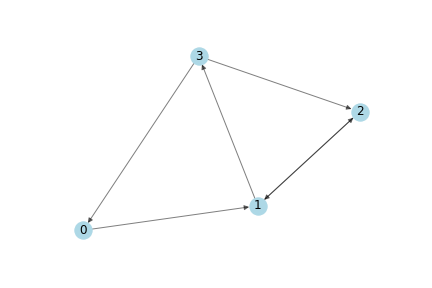
\includegraphics[scale=0.6]{graph.png}
    \caption{A simple directed graph}
    \label{fig:2_1}
\end{figure}

(a) Derive the adjacency matrix representation $A$ and degree matrix $D$. Note that in this case a node $n$ is a neighbor of node $v$ if there exists an edge from $v$ to $n$.

解: 邻接矩阵为
\begin{equation}
  A=\begin{bmatrix}
    0 & 1 & 0 & 0 \\
    0 & 0 & 1 & 1 \\
    0 & 1 & 0 & 0 \\
    1 & 0 & 1 & 0 \\
  \end{bmatrix}
\end{equation}

出度矩阵为
\begin{equation}
  D=\begin{bmatrix}
    1 & 0 & 0 & 0 \\
    0 & 2 & 0 & 0 \\
    0 & 0 & 1 & 0 \\
    0 & 0 & 0 & 2 \\
  \end{bmatrix}
\end{equation}

(b) We generate features for every node based on its index, i.e. $[i, -i]$ for node $i$.  Apply the propagation rule on adjacency matrix $A$ and input features $X$ to derive the output matrix.

解: 由题意可知输入特征为
\begin{equation}
  X=\begin{bmatrix}
    0 &  0 \\
    1 & -1 \\
    2 & -2 \\
    3 & -3 \\
  \end{bmatrix}
\end{equation}

所以, 输出矩阵为
\begin{equation}
  f(X,A)=AX
  =\begin{bmatrix}
    1 & -1 \\
    5 & -5 \\
    1 & -1 \\
    2 & -2 \\
  \end{bmatrix}
\end{equation}

(c) We found that nodes with large degrees will have large values in their feature representation while nodes with small degrees will have small values. This can cause vanishing or exploding gradients. Therefore, the feature representations can be normalized by node degree by transforming the adjacency matrix $A$ by multiplying it with the inverse degree matrix $D$. Thus our simplified propagation rule looks like this: $f(x,A) = D^{-1}AX$. We also found that the aggregated representation of a node does not include its own features. To address the problem, we add a self-loop to each node, by adding the identity matrix $I$ to the adjacency matrix $A$ before applying the propagation rule, that is, $\hat{A} = A + I$. $\hat{D}$ is the degree matrix of $\hat{A}$, i.e., the degree matrix of $A$ with forced self-loops. Derive the output matrix after normalizing the feature representations and adding self-loops.

解: 加上自回路后, 邻接矩阵为
\begin{equation}
  \hat{A}=A+I
  =\begin{bmatrix}
    1 & 1 & 0 & 0 \\
    0 & 1 & 1 & 1 \\
    0 & 1 & 1 & 0 \\
    1 & 0 & 1 & 1 \\
  \end{bmatrix}
\end{equation}

其度矩阵为
\begin{equation}
  \hat{D}=\begin{bmatrix}
    2 & 0 & 0 & 0 \\
    0 & 3 & 0 & 0 \\
    0 & 0 & 2 & 0 \\
    0 & 0 & 0 & 3 \\
  \end{bmatrix}
\end{equation}

所以, 输出矩阵为
\begin{equation}
  f(X,\hat{A})=\hat{D}^{-1}\hat{A}X
  =\begin{bmatrix}
    \frac{1}{2} & -\frac{1}{2} \\
    2 & -2 \\
    \frac{3}{2} & -\frac{3}{2} \\
    \frac{5}{3} & -\frac{5}{3} \\
  \end{bmatrix}
\end{equation}

(d) We add back the weights matrix $W$ as follows: 
$$W =\begin{bmatrix} 1 & -1 \\ -1 & 1 \end{bmatrix}.$$
Derive the output matrix.

解: 输出矩阵为
\begin{equation}
  f(X,\hat{A})=\hat{D}^{-1}\hat{A}XW
  =\begin{bmatrix}
    1 & -1 \\
    4 & -4 \\
    3 & -3 \\
    \frac{10}{3} & -\frac{10}{3} \\
  \end{bmatrix}
\end{equation}

(e) Use the same $W$ and add the ReLU activation function for $\sigma$. Derive the output matrix.

解: 输出矩阵为
\begin{equation}
  f(X,\hat{A})=\mathrm{ReLU}\left(\hat{D}^{-1}\hat{A}XW\right)
  =\begin{bmatrix}
    1 & 0 \\
    4 & 0 \\
    3 & 0 \\
    \frac{10}{3} & 0 \\
  \end{bmatrix}
\end{equation}

(f) We can apply a graph convolutional network on a real graph, Zachary's karate club. Zachary's karate club is a commonly used social network where nodes represent members of a karate club and the edges their mutual relations. While Zachary was studying the karate club, a conflict arose between the administrator and the instructor which resulted in the club splitting in two. The figure below shows the graph representation of the network and nodes are labeled according to which part of the club. The administrator and instructor are marked with `A' and `I', respectively.

\begin{figure}[ht]
  \centering
  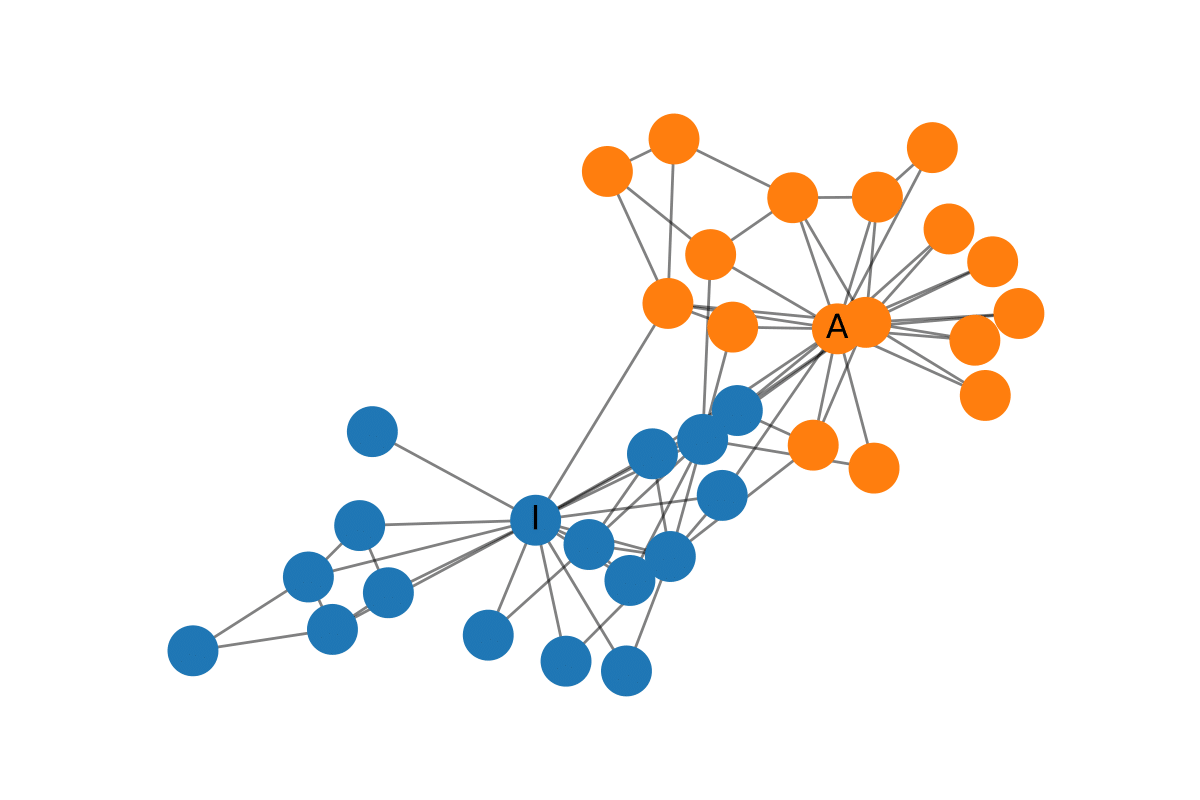
\includegraphics[scale=0.22]{club.png}
  \caption{Zachary's Karate Club}
  \label{fig:2_2}
\end{figure}

You can use the following python codes to get the dataset:

\verb|from networkx import karate_club_graph|

\verb|zkc = karate_club_graph()|

Design a GNN to separate communities in Zachary's Karate Club. We here use just the identity matrix as input representation, that is, each node is represented as a one-hot encoded variable. Show the final output feature representations for the nodes of Figure \ref{fig:2_2}. 

\emph{Hint:} Please try a GCN with two hidden layers just like (e), and initialize the weights randomly, then extract the feature representations and plot them. You will find even randomly initialized GCNs can separate communities in Zachary's Karate Club. Next, you can try your own GNN for better performance.

解: 首先绘制 Zachary's Karate Club 如图 \ref{fig:zkc_init} 所示, 其中标号 0 的节点对应 `I', 标号 33 的节点对应 `A'.

\begin{figure}[htbp]
  \centering
  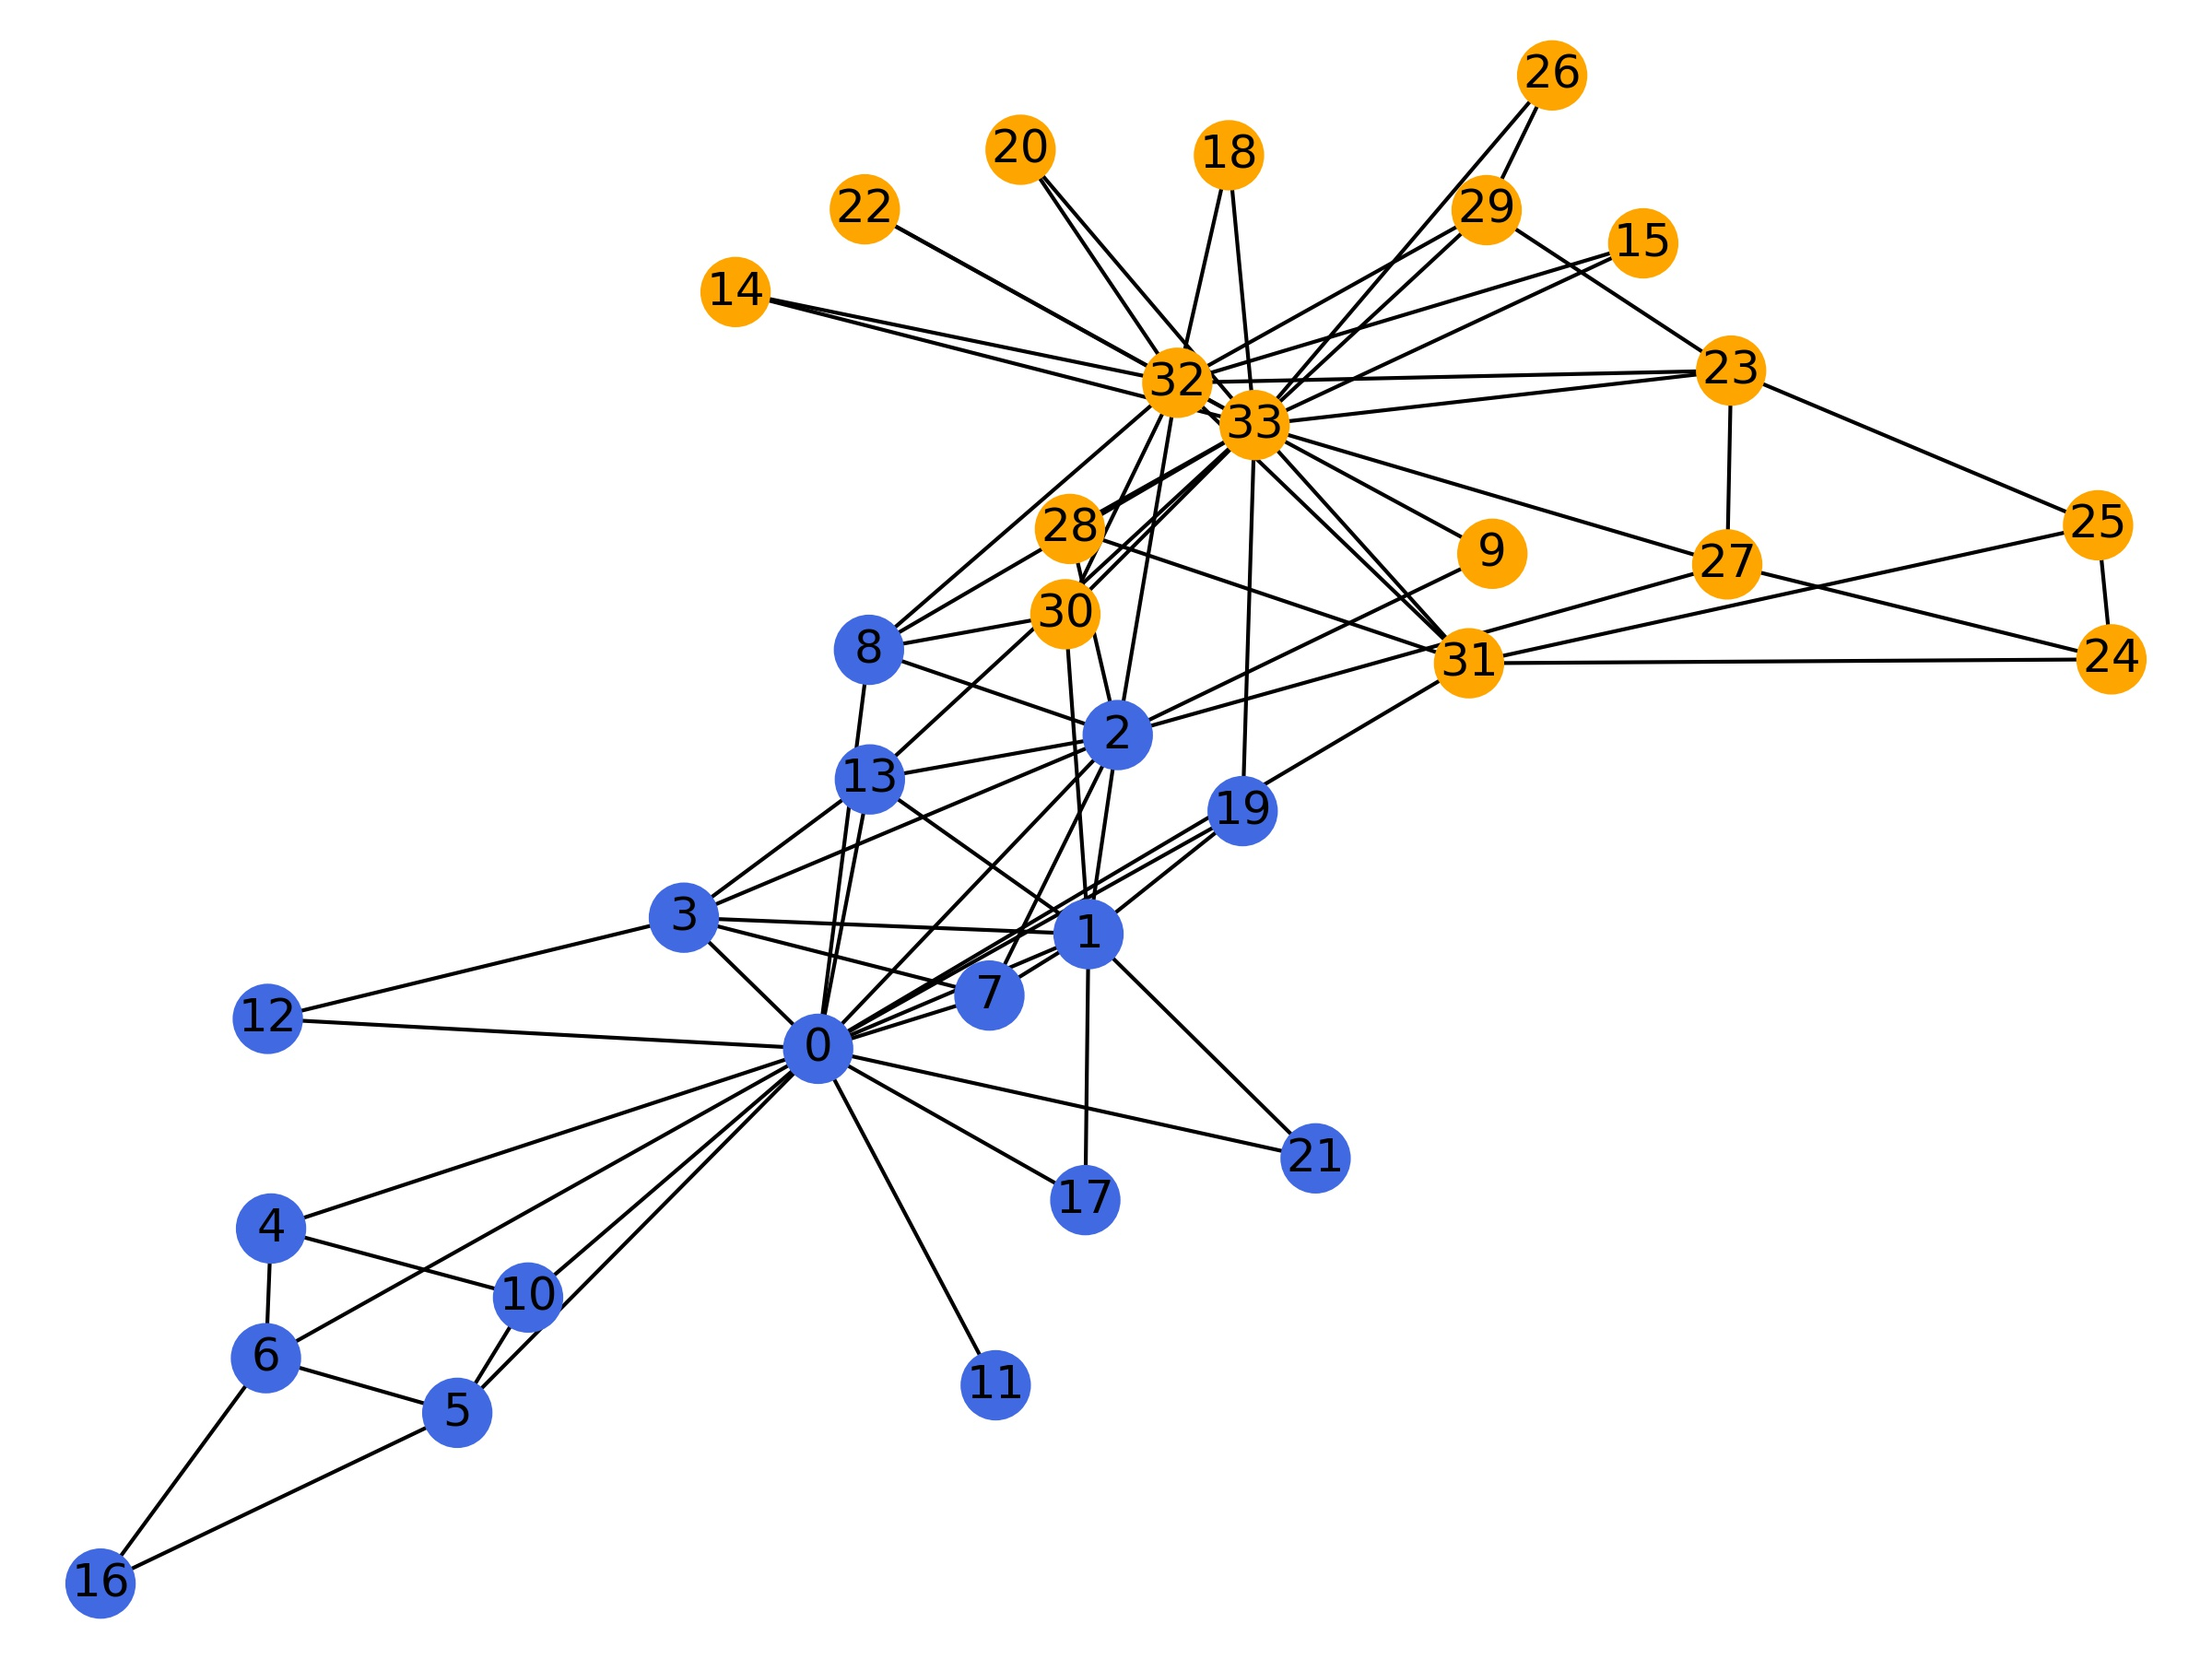
\includegraphics[width=12cm]{zkc_init.jpg}
  \caption{Zachary's Karate Club}
  \label{fig:zkc_init}
\end{figure}

与 (e) 类似, $H^0=I$, 建立两层 GCN 网络, 
\begin{equation}
  \begin{aligned}
    H^1 &=\mathrm{ReLU}(\hat{D}^{-1}\hat{A}H^0W^0)\\
    H^2 &=\mathrm{ReLU}(\hat{D}^{-1}\hat{A}H^1W^1)\\
  \end{aligned}
\end{equation}

随机初始化权重矩阵 $W^0,W^1$ 进行计算, 经过数次尝试, 得到 Zachary's Karate Club 的特征表示如图 \ref{fig:zkc_gcn} 所示, 由图可知即便是随机初始化的权重矩阵也可以将两个类别分开.

\begin{figure}[htbp]
  \centering
  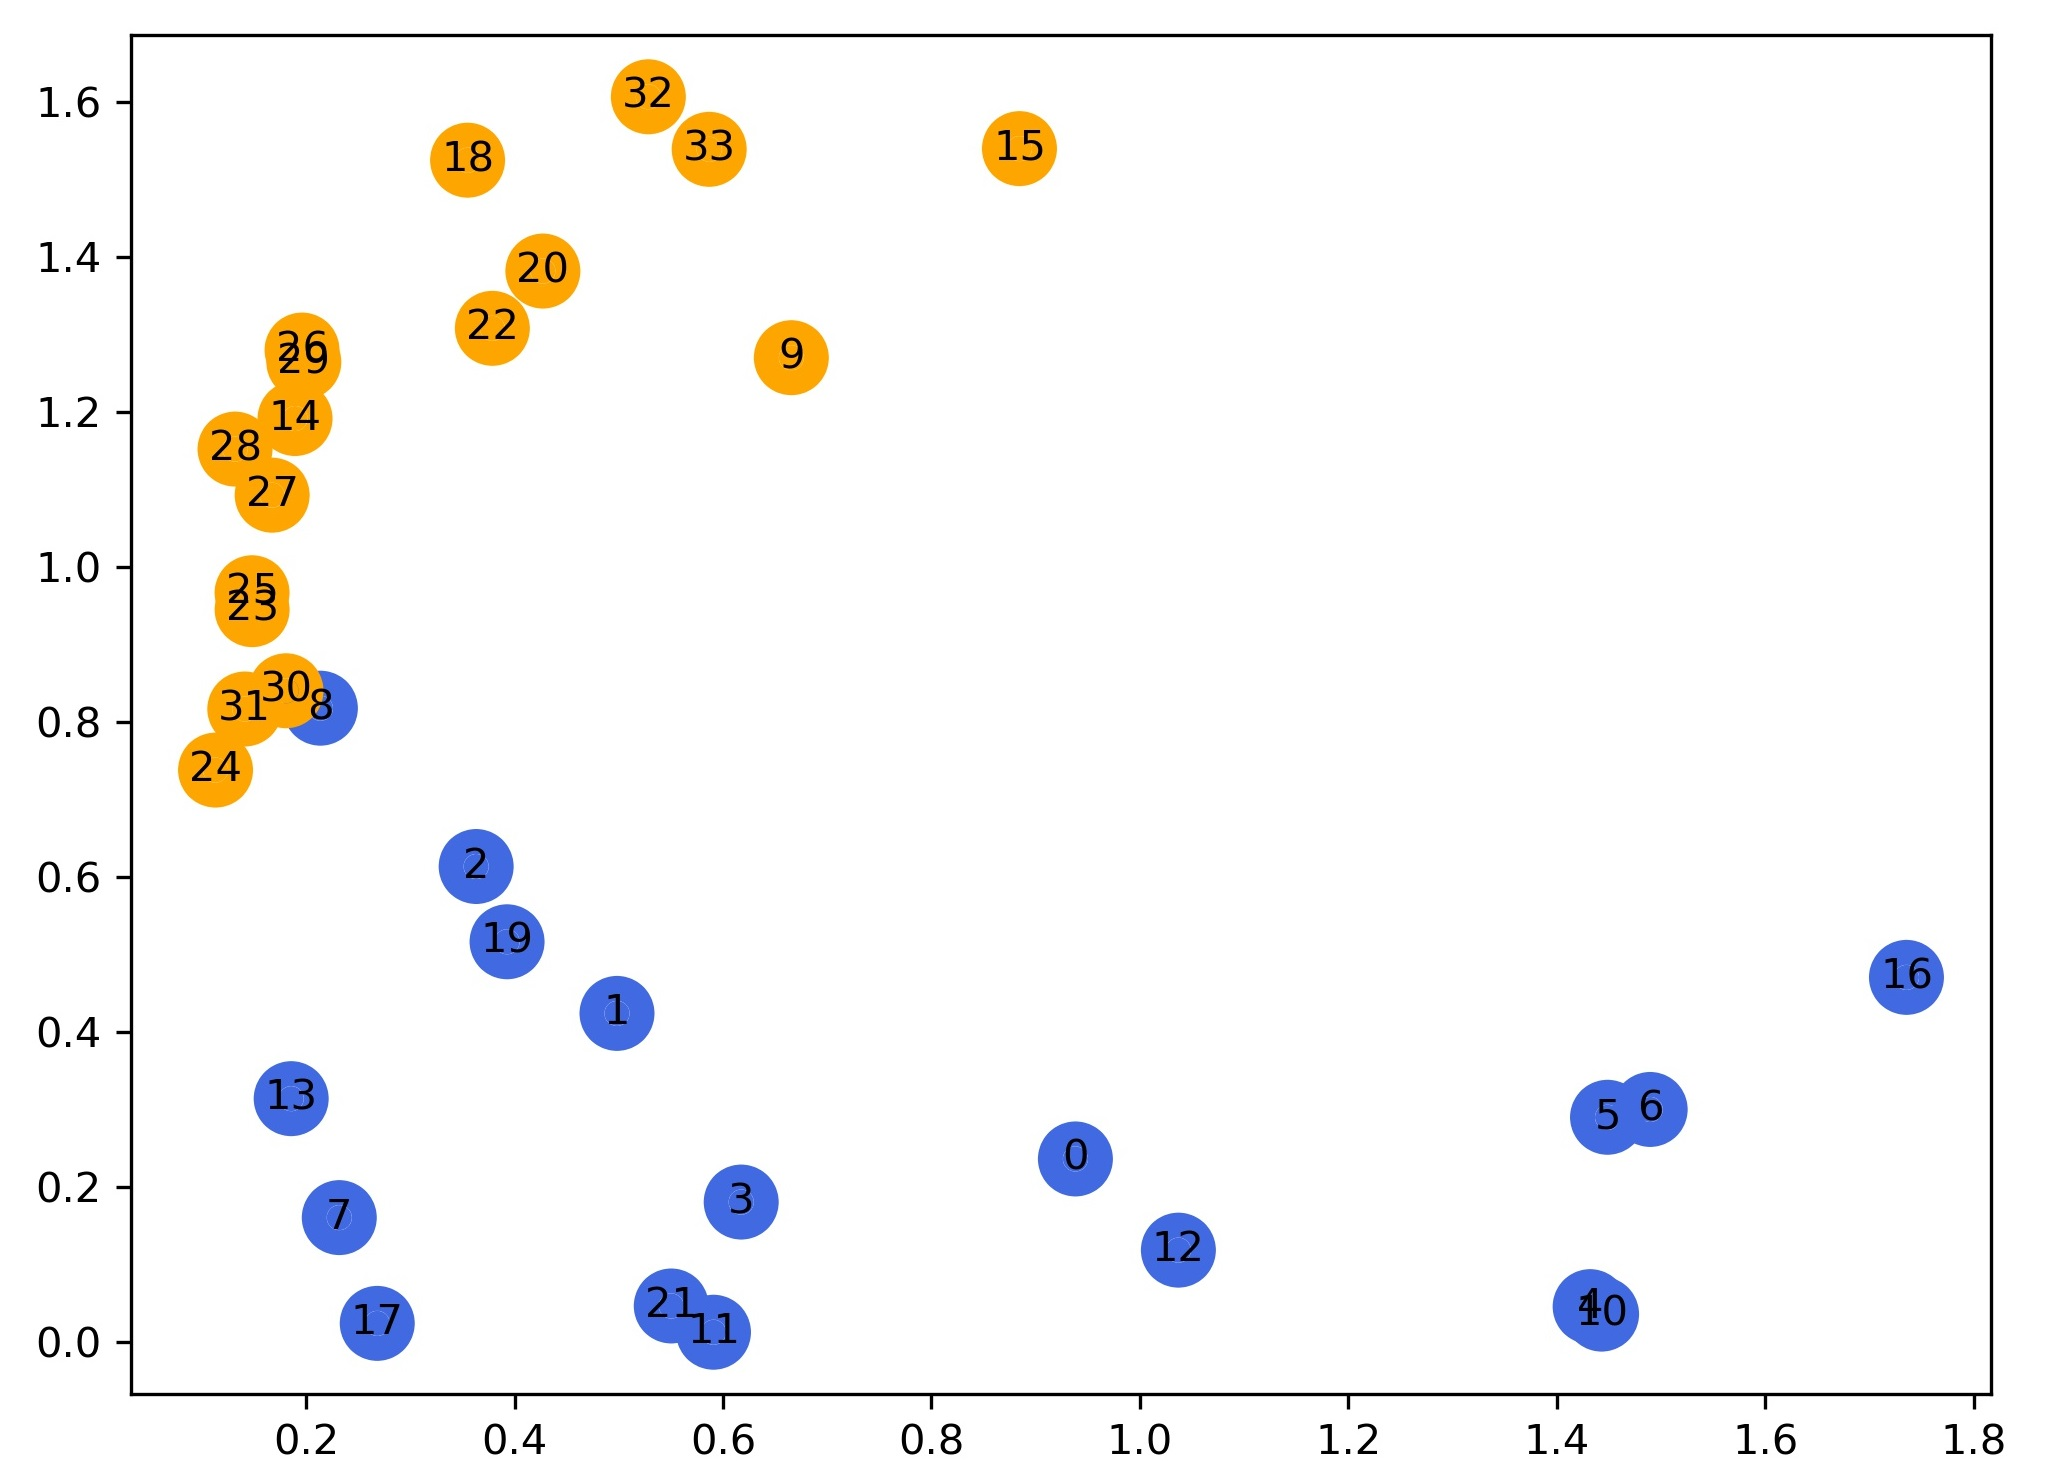
\includegraphics[width=12cm]{zkc_gcn.jpg}
  \caption{Feature Representations of Zachary's Karate Club}
  \label{fig:zkc_gcn}
\end{figure}

\section*{Programming: Decision Tree}

实现决策树算法 C4.5,并且在 \emph{Sogou Corpus} 数据集上测试它的效果(数据集详情见 readme). 

要求:
\begin{itemize}
  \item 不能调用已有的机器学习包
  \item 将数据随机分为 3:1:1 的三份,分别为训练集,交叉验证集,测试集。请在训练集上训练,交叉验证集上选择超参数,用选出的最好模型在测试集上给出测试结果。因此,在报告中需要说明算法的超参数有哪些,在不同的超参数设置下训练集和交叉验证集的分类正确率,最好模型的超参数设置,以及最后的测试正确率。
  \item 请结构化代码,必须包含但不限于如下几个函数(请从代码中分离出来,有明确的这几个函数,函数参数可以有所变化):
  \begin{itemize}
    \item \textbf{main()}

      要求main函数在运行中,逐个测试不同的超参数,然后打印出每个超参数的设置,该设置下的训练、验证正确率(就是上面第二点中提到的要出现在报告中的结果)。

    \item \textbf{GenerateTree(args)}

        生成树的总代码,\emph{args} 为各种超参数,包括但不限于下面的 \emph{thresh},或者其他会影响树性能的超参数,自由发挥。

    \item \textbf{SplitNode(samplesUnderThisNode, thresh, \dots)}

        对当前节点进行分支,\emph{samplesUnderThisNode} 是当前节点下的样本,\emph{thresh} 是停止分支的阈值,停止分支的条件请在实验报告中说明。

    \item \textbf{SelectFeature(samplesUnderThisNode, \dots)}

        对当前节点下的样本,选择待分特征。

    \item \textbf{Impurity(samples)}

        给出样本 \emph{samples} 的不纯度,请在实验报告中说明采用的不纯度度量。

    \item \textbf{Decision(GeneratedTree, XToBePredicted)}

        使用生成的树 \emph{GenerateTree},对样本 \emph{XToBePredicted} 进行预测。

    \item \textbf{Prune(GeneratedTree, CorssValidationDataset, \dots)}

        对生成好的树 \emph{GeneratedTree}(已经过 stopped splitting) 进行剪枝:考虑所有相邻的叶子节点,如果将他们消去可以增加验证集上的正确率,则减去两叶子节点,将他们的共同祖先作为新的叶子节点。或者实现其他的剪枝方法,如有,请在实验报告中说明。

  \end{itemize}

\end{itemize}

解: 数据集采用均匀分布随机分割为 3:1:1 的三份, 详见函数 \verb|split()|, 分割结果见 

\hspace{4cm}\verb|train_split.txt|, \verb|validate_split.txt|, \verb|test_split.txt|.

算法的超参数为分枝不纯度下降的阈值 (threshold), 设置为列表 [0.5, 0.4, 0.3, 0.2, 0.1, 0.09, 0.08, 0.07, 0.06, 0.05, 0.04, 0.03, 0.02, 0.01, 0.005, 0.003, 0.001], 停止分枝的条件为当前节点的数据纯净 (pure), 或者按任何特征进行分割都不能使得不纯度下降大于阈值, 其中不纯度采用熵不纯度 (entropy impurity) 进行度量. 算法采用的剪枝方法为 C4.5 基于规则的算法, 即把生成的决策树转化为等价的规则集合, 剪去任何一个可以使某个规则在验证集上分类正确率上升的前件 (precondition), 直到无法剪除, 最后将规则按分类正确率从高到低排序.

在不同的超参数设置下训练集, 交叉验证集和测试集的分类正确率如表 \ref{tab:train_validate_acc} 所示, 当阈值 $\text{threshold}\ls0.01$ 时, 验证集正确率不再改变, 最佳参数 $\text{threshold}=0.01$ 下最佳模型的测试正确率为 $\text{accuracy}=0.77701$.

\begin{table}[htbp]
  \centering
  \caption{不同阈值训练集, 交叉验证集和测试集正确率}
  \label{tab:train_validate_acc}
  \begin{tabular}{cccc}
    \toprule
    threshold & train accuracy & validate accuracy & test accuracy \\
    \midrule
    0.5       & 0.11498        & 0.10131           & 0.10942      \\
    0.4       & 0.11498        & 0.10131           & 0.10942      \\
    0.3       & 0.11498        & 0.10131           & 0.10942      \\
    0.2       & 0.42276        & 0.41247           & 0.41828      \\
    0.1       & 0.78746        & 0.76844           & 0.73615      \\
    0.09      & 0.80523        & 0.79221           & 0.74965      \\
    0.08      & 0.80708        & 0.79428           & 0.74931      \\
    0.07      & 0.84251        & 0.83356           & 0.77701      \\
    0.06      & 0.84286        & 0.83425           & 0.77701      \\
    0.05      & 0.84402        & 0.83494           & 0.77909      \\
    0.04      & 0.84634        & 0.83494           & 0.77666      \\
    0.03      & 0.84599        & 0.8346            & 0.77666      \\
    0.02      & 0.84611        & 0.83494           & 0.77666      \\
    0.01      & 0.84541        & 0.83563           & 0.77701      \\
    0.005     & 0.84483        & 0.83563           & 0.77666      \\
    0.003     & 0.84483        & 0.83563           & 0.77666      \\
    0.001     & 0.84483        & 0.83563           & 0.77666 \\
    \bottomrule       
  \end{tabular}
\end{table}

训练集正确率, 交叉验证集正确率和测试集正确率与阈值变化关系分别如图 \ref{fig:train}, 图 \ref{fig:cross_validation} 和图 \ref{fig:test} 所示, 可见使用 C4.5 的方法, 模型的分类正确率基本随着阈值的减小而逐渐升高, 最后逐渐收敛趋于不变.

\begin{figure}[htbp]
  \centering
  \begin{minipage}[t]{0.48\textwidth}
    \centering
    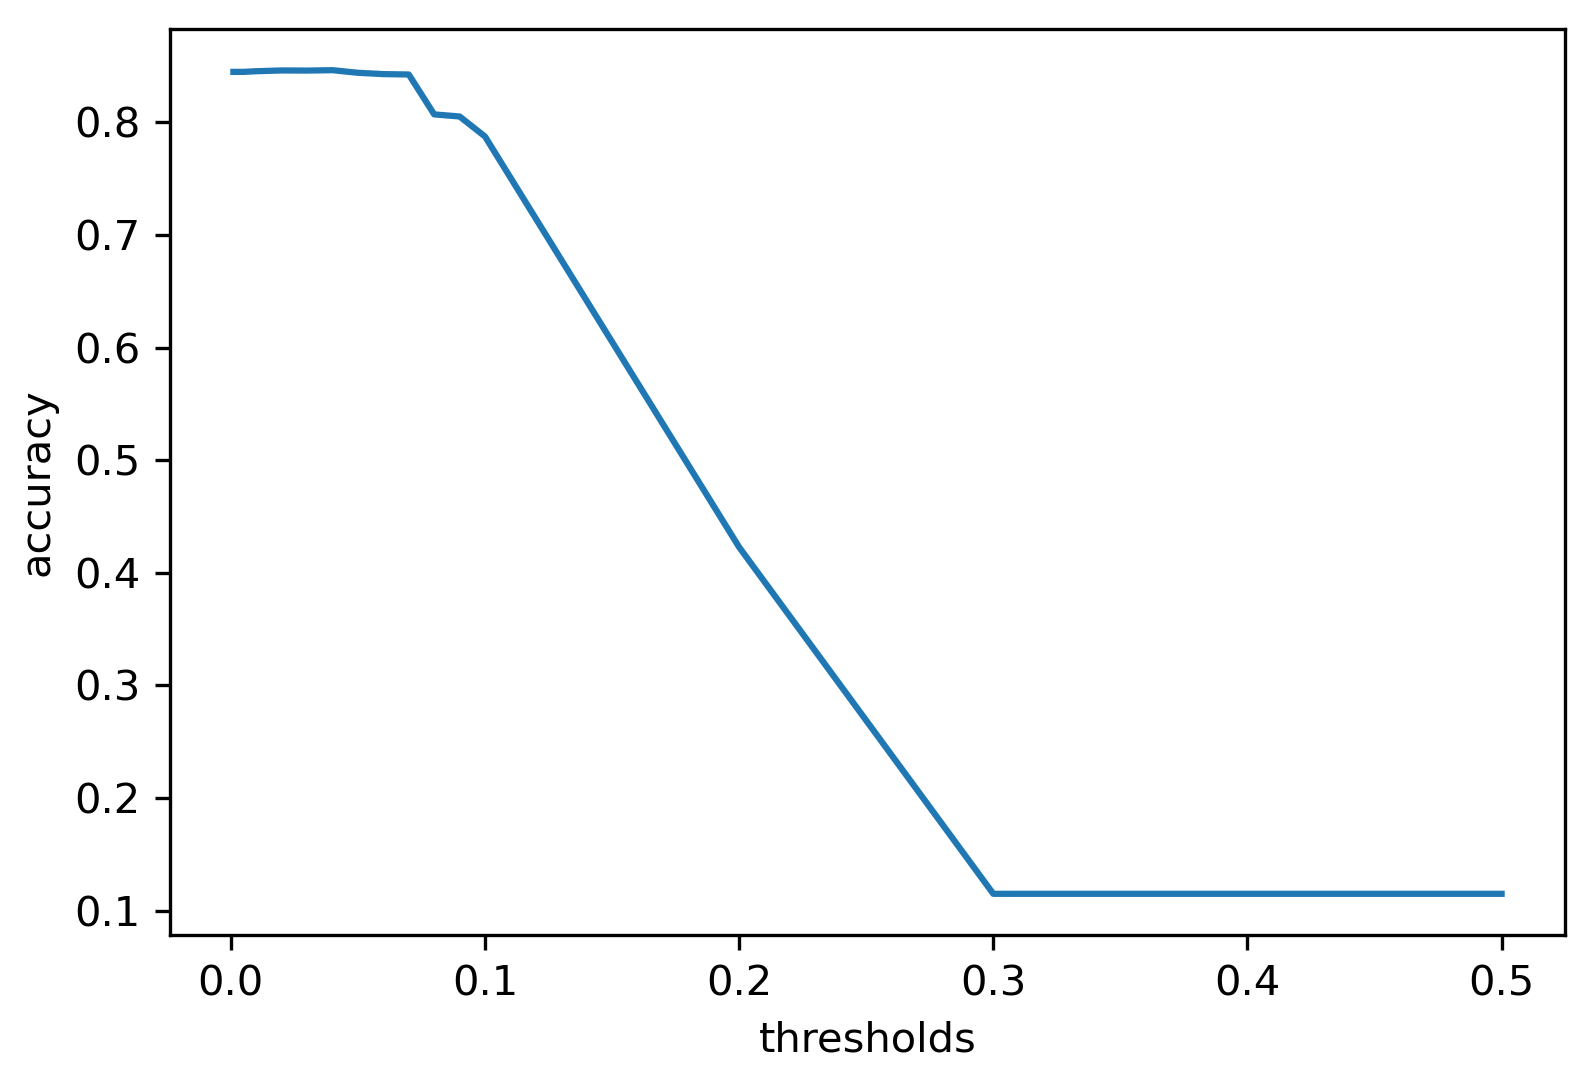
\includegraphics[width=8cm]{train.png}
    \caption{训练集正确率与阈值变化关系}
    \label{fig:train}
  \end{minipage}
  \begin{minipage}[t]{0.48\textwidth}
    \centering
    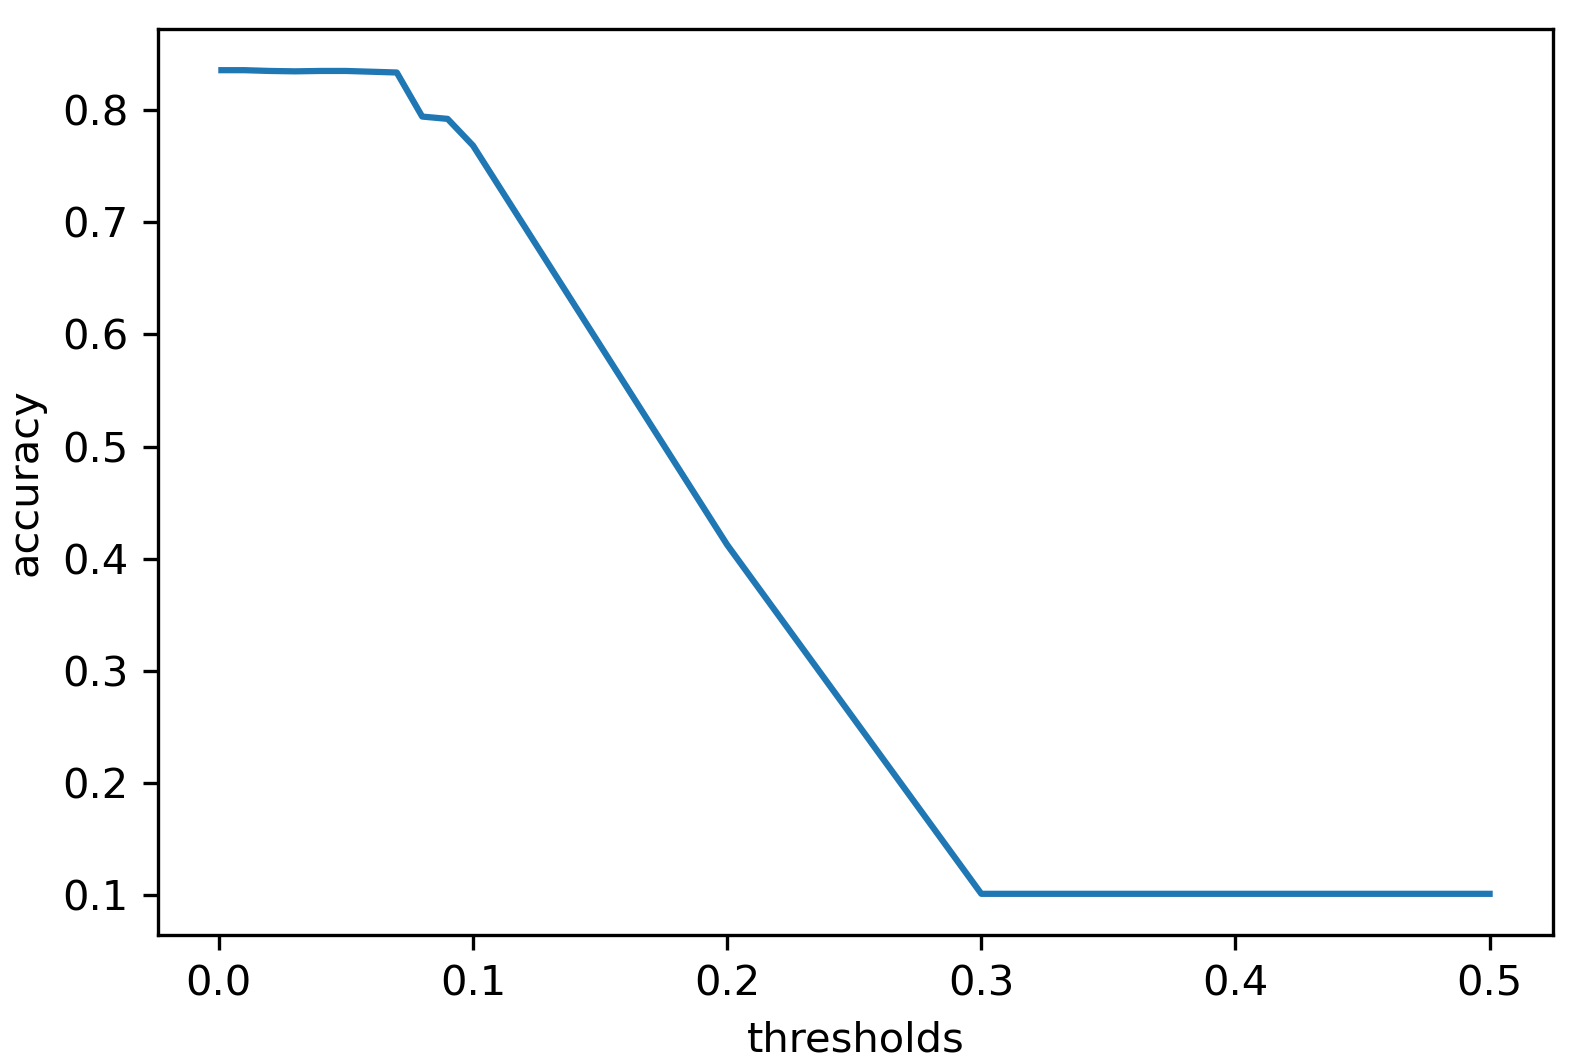
\includegraphics[width=8cm]{cross_validation.png}
    \caption{交叉验证集正确率与阈值变化关系}
    \label{fig:cross_validation}
  \end{minipage}
\end{figure}

\begin{figure}
  \centering
  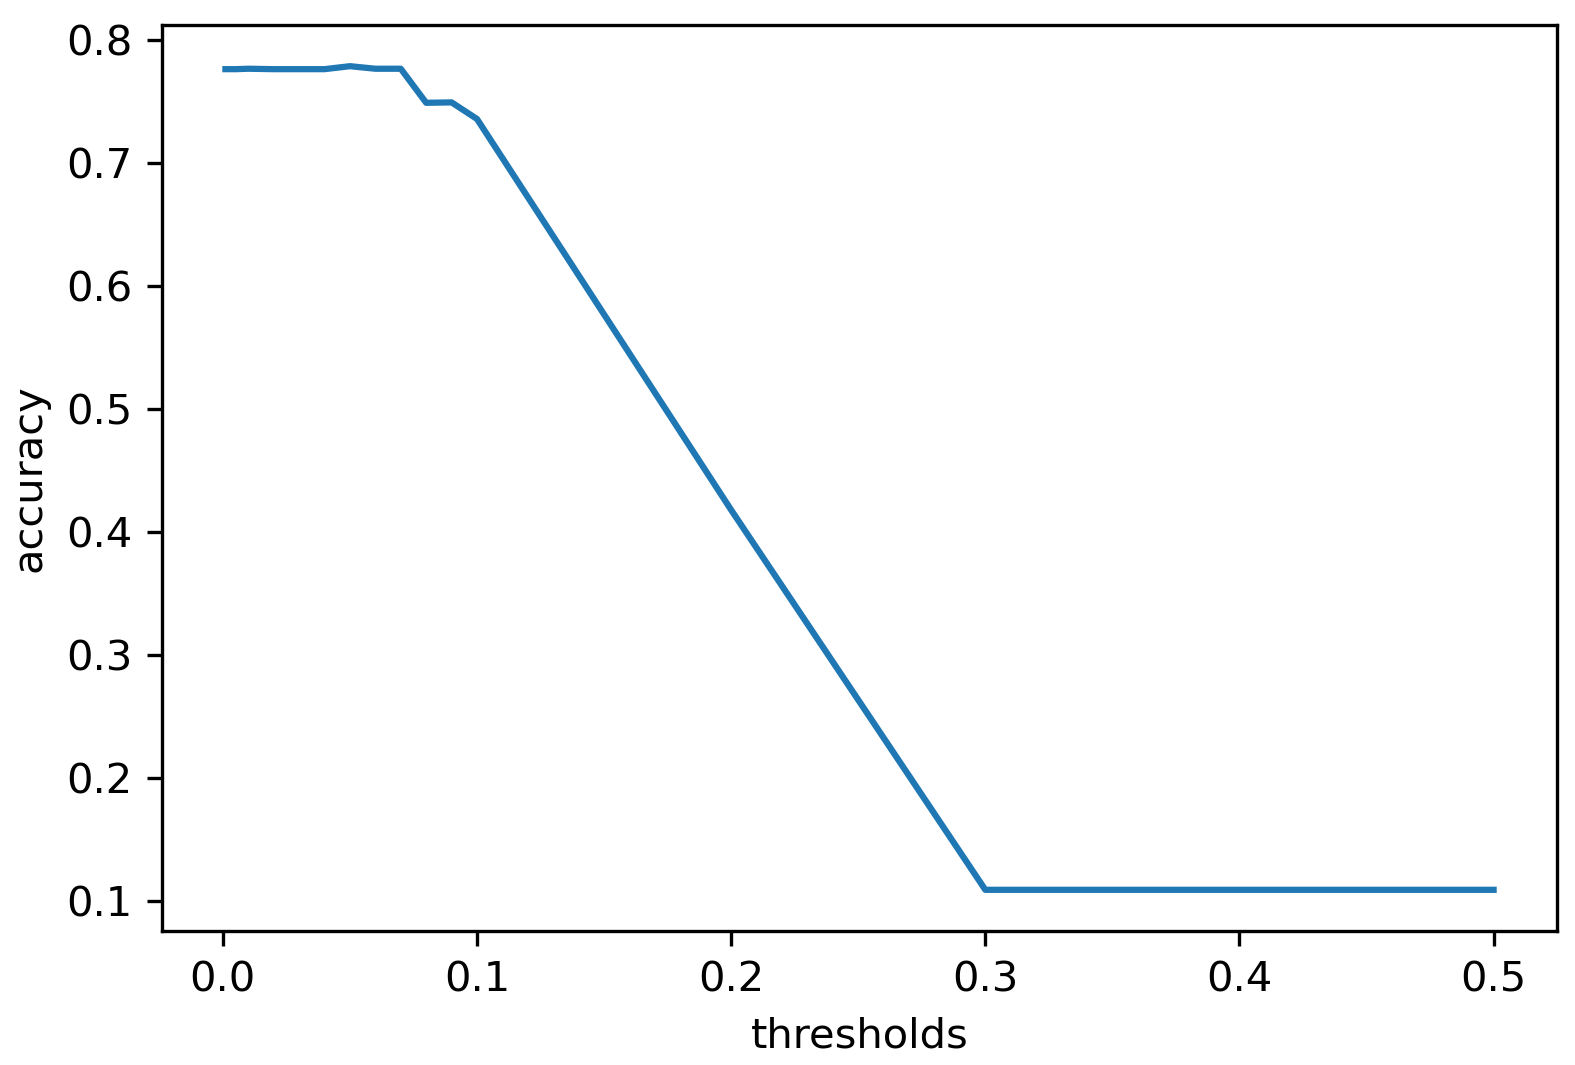
\includegraphics[width=12cm]{test.png}
  \caption{测试集正确率与阈值变化关系}
  \label{fig:test}
\end{figure}

% Reference
% \begin{thebibliography}{1}

% \bibitem{lle}

% Sam T. Roweis, lle.m - A simple matlab routine to perform LLE, Locally Linear Embedding (LLE) Code Page, \url{https://cs.nyu.edu/~roweis/lle/code.html}.

% \end{thebibliography}

\end{document}
